\chapter{Teoría de grafos}
    Antes de comenzar con el estudio de las redes de transporte público, y con el fin de partir desde bases bien fundamentadas, vamos a introducir una serie de definiciones en torno a la teoría de grafos. En este caso nos importa fundamentar adecuadamente qué es un \textit{camino} en el contexto de esta teoría, lo que nos ayudará a tener un formalismo de lo que es una ruta de transporte público. Asimismo, nos interesa explorar cómo la noción de camino nos ayuda a entender la estructura de una red. Para esto también estudiaremos el concepto de \textit{centralidad}, que nos ayudará a evaluar la importancia que tiene un determinado nodo en el contexto del resto del grafo. Finalmente, gracias a lo anterior, estudiaremos distintos algoritmos para lograr encontrar caminos óptimos entre cualesquiera dos nodos.

    Los problemas de movilidad urbana requieren modelos que abstraigan la complejidad de la ciudad sin perder los elementos esenciales de conectividad. La \emph{teoría de grafos} provee justamente ese andamiaje formal: reduce las interacciones físicas a vértices y aristas y, a partir de ahí, permite cuantificar eficiencia, robustez y vulnerabilidad de toda la red (Rodrigues, 2013).

    Este capítulo se basa en \cite{diestel2017} y \cite{bangjensen2007}.

    \subsection{Definición y conceptos básicos}

        \begin{definicion}
            Un \textbf{grafo} $G$ es un par $(V,E)$ que consiste en un conjunto no vacío $V$ de \textbf{vértices} (o \textbf{nodos}) y un conjunto $E$ de subconjuntos de 2 elementos de $V$, denominados \textbf{aristas}.
        \end{definicion}

    A un grafo $G$ con conjunto de aristas $V$ también lo podemos definir como un grafo \textit{en} $V$ o simplemente $G(V)$ \cite{diestel2017}.

    \begin{definicion}
        Llamamos \textit{orden} de un grafo G al número de vértices que contiene y lo representamos como $|G|$. A la cantidad de aristas de $G$ la escribiremos como $\parallel G \parallel$. Un grafo puede ser \textit{finito} o \textit{infinito}.
    \end{definicion}

    \begin{ejemplo}
        La forma habitual de representar un grafo es dibujando un punto por cada vértice y uniendo dichos puntos con una línea si el par correspondiente forma una arista. La disposición de los puntos y las líneas es irrelevante; lo único que importa es qué pares de vértices están conectados.

        \begin{figure}[ht]
            \centering
            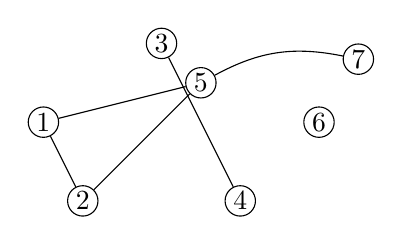
\begin{tikzpicture}
                % nodes
                \node[draw, circle, inner sep=1pt] (1) at (0,1) {1};
                \node[draw, circle, inner sep=1pt] (2) at (0.5,0) {2};
                \node[draw, circle, inner sep=1pt] (3) at (1.5,2) {3};
                \node[draw, circle, inner sep=1pt] (4) at (2.5,0) {4};
                \node[draw, circle, inner sep=1pt] (5) at (2,1.5) {5};
                \node[draw, circle, inner sep=1pt] (6) at (3.5,1) {6};
                \node[draw, circle, inner sep=1pt] (7) at (4,1.8) {7};
                % edges
                \draw (1) -- (2);
                \draw (1) -- (5);
                \draw (2) -- (5);
                \draw (3) -- (4);
                \draw (5) to[bend left=20] (7);
            \end{tikzpicture}
            \caption{Ejemplo de un grafo con $V=\{1, ..., 7\}$ y $E=\{\{1,2\}, \{1,5\}, \{2,5\}, \{3,4\}, \{5,7\}\}$.}
            \label{fig:ejemplo-grafo}
        \end{figure}


        El grafo $G$ tiene el orden $|G|=7$ y el número de aristas $\parallel G \parallel = 5$.
    \end{ejemplo}

    En el resto de este trabajo asumiremos que todos los grafos son finitos.

    \subsection{Tipos de grafos}

        Ahora que sabemos lo que es un grafo, es pertinente preguntarnos si es posible clasificarlos. Aunque posible, la clasificación de los grafos es una tarea multifacética que puede atender a una diversidad de criterios. Es posible categorizarlos, por ejemplo, en función de su estructura general (como en el caso de los grafos planares, bipartitos o completos), de las propiedades de conectividad que exhiben, o incluso de la presencia de ciclos. No obstante, para los fines de esta introducción, nos centraremos en una de las distinciones más fundamentales, la cual emana directamente de las propiedades inherentes al conjunto de aristas $E$. Específicamente, exploraremos la clasificación de los grafos según si sus aristas poseen una dirección definida (grafos dirigidos y no dirigidos) y si se les atribuye un valor numérico (grafos ponderados).

        Estas propiedades dan lugar a un espectro de categorías de grafos, cada una con implicaciones estructurales y algorítmicas particulares. Por consiguiente, a continuación se presentan las definiciones formales:

        \begin{definicion}[Grafo no dirigido]
            Un grafo es \textbf{no dirigido} si sus aristas no tienen una orientación específica; es decir, $(u, v) \in E$ implica que $(v, u) \in E$.
        \end{definicion}

        \begin{ejemplo}
            A continuación se muestra un ejemplo de grafo no dirigido:

            \begin{center}
                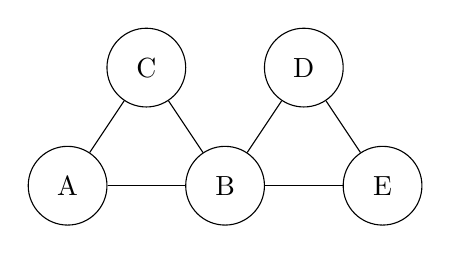
\begin{tikzpicture}[scale=1, every node/.style={draw, circle, minimum size=1cm}]
                    \node (A) at (0,0) {A};
                    \node (B) at (2,0) {B};
                    \node (C) at (1,1.5) {C};
                    \node (D) at (3,1.5) {D};
                    \node (E) at (4,0) {E};

                    \draw (A) -- (B);
                    \draw (A) -- (C);
                    \draw (B) -- (C);
                    \draw (B) -- (D);
                    \draw (B) -- (E);
                    \draw (D) -- (E);
                \end{tikzpicture}
            \end{center}
        \end{ejemplo}

        \begin{definicion}[Grafo dirigido (dígrafo)]
            Un grafo es \textbf{dirigido} (o \emph{dígrafo}) si cada arista tiene una dirección; es decir, $(u, v) \in E$ no implica que $(v, u) \in E$ (aunque puede ocurrir). En este caso, diremos que $u$ se dirige a $v$.
        \end{definicion}

        \begin{ejemplo}
            Ejemplo de grafo dirigido:

            \begin{center}
                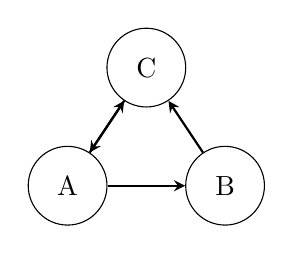
\begin{tikzpicture}[scale=1, every node/.style={draw, circle, minimum size=1cm}, >=stealth]
                    \node (A) at (0,0) {A};
                    \node (B) at (2,0) {B};
                    \node (C) at (1,1.5) {C};

                    \draw[->, thick] (A) -- (B);
                    \draw[->, thick] (B) -- (C);
                    \draw[->, thick] (C) -- (A);
                    \draw[->, thick] (A) -- (C);
                \end{tikzpicture}
            \end{center}
        \end{ejemplo}

        \begin{definicion}[Grafo ponderado]
            Un grafo es \textbf{ponderado} si a cada arista $(u, v) \in E$ se le asigna un peso $w(u, v) \in \mathbb{R}$ que representa costos, distancias u otra métrica relevante. Un grafo puede ser ponderado además de dirigido o no dirigido.
        \end{definicion}

        \begin{ejemplo}
            Ejemplo de grafo ponderado:

            \begin{center}
                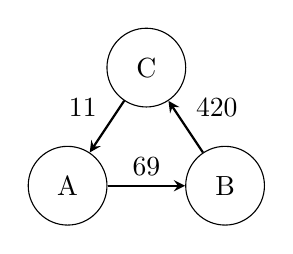
\begin{tikzpicture}[scale=1, vertex/.style={draw, circle, minimum size=1cm}, >=stealth]
                    % Definición de vértices
                    \node[vertex] (A) at (0,0) {A};
                    \node[vertex] (B) at (2,0) {B};
                    \node[vertex] (C) at (1,1.5) {C};

                    % Aristas con etiquetas
                    \draw[->, thick] (A) -- node[above, draw=none, fill=none] {69} (B);
                    \draw[->, thick] (B) -- node[above right, draw=none, fill=none] {420} (C);
                    \draw[->, thick] (C) -- node[above left, draw=none, fill=none] {11} (A);
                \end{tikzpicture}
            \end{center}
        \end{ejemplo}

    \subsection{Propiedades fundamentales de los grafos}

        Los grafos poseen diversas propiedades matemáticas que permiten su análisis estructural. Algunas que son especialmente valiosas para el presente estudio son la \textit{conectividad}, los \textit{caminos}, los \textit{ciclos}, y las representaciones matriciales como la matriz de adyacencia.

        \begin{definicion}[Adyacencia de nodos]
            Sean $G = (V, E)$ un grafo y $u, v \in V$ dos nodos distintos.
            Se dice que $u$ y $v$ son \textbf{adyacentes} si existe una arista que los conecta directamente, es decir:
            \begin{itemize}
                \item En un grafo no dirigido, $u$ y $v$ son adyacentes si $(u, v) \in E$ (lo que implica también $(v, u) \in E$).
                \item En un grafo dirigido, $u$ es adyacente a $v$ si $(u, v) \in E$ (pero no necesariamente $(v, u) \in E$).
            \end{itemize}
            De forma equivalente, dos nodos son adyacentes si la entrada correspondiente en la matriz de adyacencia $A$ es distinta de cero, es decir, $a_{uv} \neq 0$.
        \end{definicion}

        \begin{definicion}[Subgrafo]
            Un \textbf{subgrafo} $H = (V_H, E_H)$ de un grafo $G = (V, E)$ es un grafo tal que $V_H \subseteq V$ y $E_H \subseteq E$. Es decir, un subgrafo es una parte de un grafo que mantiene la estructura de nodos y aristas del grafo original.
        \end{definicion}

        \begin{ejemplo}
            Ejemplo de subgrafo:

            \begin{center}
                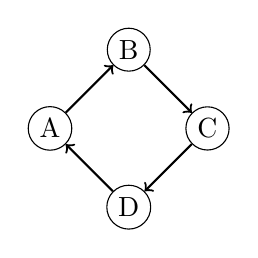
\begin{tikzpicture}[scale=1, every node/.style={circle, draw, fill=white, inner sep=2pt}]
                    \node (a) at (0,0) {A};
                    \node (b) at (1,1) {B};
                    \node (c) at (2,0) {C};
                    \node (d) at (1,-1) {D};
                    \draw[->, thick] (a) -> (b);
                    \draw[->, thick] (b) -> (c);
                    \draw[->, thick] (c) -> (d);
                    \draw[->, thick] (d) -> (a);
                \end{tikzpicture}
            \end{center}
        \end{ejemplo}

        \begin{definicion}[Camino]
            Un \textbf{camino} en un grafo $G$ es una sucesión de vértices $P_k = (v_1, v_2, \dots, v_k)$ tal que $\{v_i, v_{i+1}\} \in E$ para todo $i \in \{1, \dots, k-1\}$ y ningún vértice se repite.
        \end{definicion}

        \begin{ejemplo}
            Ejemplo de camino:

            \begin{center}
                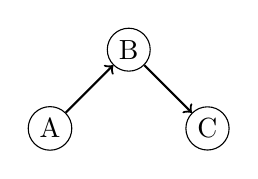
\begin{tikzpicture}[scale=1, every node/.style={circle, draw, fill=white, inner sep=2pt}]
                    \node (a) at (0,0) {A};
                    \node (b) at (1,1) {B};
                    \node (c) at (2,0) {C};
                    \draw[->, thick] (a) -> (b);
                    \draw[->, thick] (b) -> (c);
                \end{tikzpicture}
            \end{center}
        \end{ejemplo}

        \begin{definicion}[Ciclo]
            Un \textbf{ciclo} es un camino $C_k = (v_1, v_2, \dots, v_k, v_1)$ tal que el primer y el último vértice coinciden ($v_1 = v_{k+1}$) y las aristas cumplen $\{v_i, v_{i+1}\} \in E$ para $i = 1, \dots, k$.
        \end{definicion}

        \begin{ejemplo}
            Ejemplo de ciclo:

            \begin{center}
                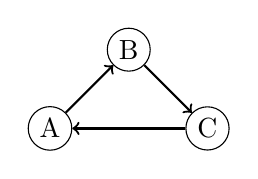
\begin{tikzpicture}[scale=1, every node/.style={circle, draw, fill=white, inner sep=2pt}]
                    \node (a) at (0,0) {A};
                    \node (b) at (1,1) {B};
                    \node (c) at (2,0) {C};
                    \draw[->, thick] (a) -> (b);
                    \draw[->, thick] (b) -> (c);
                    \draw[->, thick] (c) -> (a);
                \end{tikzpicture}
            \end{center}
        \end{ejemplo}

        \begin{definicion}[Matriz de adyacencia]
            Dado un grafo $G=(V,E)$ con $N$ nodos, la \textbf{matriz de adyacencia} es una matriz $A \in \mathbb{R}^{N \times N}$ donde cada elemento $a_{ij}$ indica si existe una conexión directa entre el nodo $i$ y el nodo $j$:
            \[
            a_{ij} =
            \begin{cases}
            1, & \text{si existe una arista entre } i \text{ y } j,\\
            0, & \text{en caso contrario.}
            \end{cases}
            \]
            En grafos ponderados, cada $a_{ij}$ toma el valor del peso asignado a la conexión.
        \end{definicion}

    \subsection{Propiedades estructurales}

    Entre las propiedades clásicas que describen la forma en que los vértices se relacionan destacan:
    \begin{itemize}
        \item \textbf{Conectividad}: existe al menos un camino entre cada par de vértices; de lo contrario la red se fragmenta en componentes conexas.
        \item \textbf{Árbol}: grafo conexo sin ciclos. Satisface $|E|=|V|-1$.
        \item \textbf{Diámetro}: longitud del camino más largo entre los caminos más cortos de todos los pares $(u,v)$.
        \item \textbf{Nodo articulación} e \textbf{istmo}: suprimirlos incrementa el número de componentes, evidencia fragilidad local. (Rodrigues, 2013).
        \item \textbf{Número de ciclos independientes}: $\mu = |E|-|V|+p$, donde $p$ es el número de componentes.
    \end{itemize}

    \subsubsection*{Nivel de red}

    \begin{description}

    \item[Índice $\beta$ (conectividad).]
    Mide cuántas aristas existen respecto al número de nodos, es decir, cuántas conexiones “promedio” puede esperar cada vértice. Valores cercanos a $1$ indican una topología arborescente (pocas alternativas de ruta), mientras que valores crecientes reflejan una mayor interconexión y, por tanto, más opciones de recorrido.
    \begin{center}
    $\displaystyle \beta \;=\; \frac{|E|}{|V|}$
    \end{center}

    \item[Índice $\alpha$ (redundancia).]
    Cuantifica la proporción de ciclos efectivamente presentes frente al máximo posible en un grafo planar. Sirve para valorar la resiliencia de la red: cuanto más alto, más caminos alternativos existen ante fallos o congestión. El parámetro $p$ indica el número de componentes conexas (en la práctica, $p=1$ si la red está totalmente conectada).
    \begin{center}
    $\displaystyle \alpha \;=\; \frac{|E| - |V| + p}{\,2|V| - 5\,}$
    \end{center}

    \item[Índice $\gamma$ (densidad planar).]
    Expresa la fracción de aristas observadas con respecto al límite superior para un grafo planar simple ($3|V|-6$). Un $\gamma$ cercano a $1$ denota que la red se aproxima a la máxima densidad planar, mientras que valores bajos sugieren poca malla y mayor fragilidad estructural.
    \begin{center}
    $\displaystyle \gamma \;=\; \frac{|E|}{\,3|V| - 6\,}$
    \end{center}

    \item[Longitud total.]
    Es la suma de las longitudes físicas de todas las aristas—por ejemplo, la distancia vial o la duración promedio del trayecto—y constituye un indicador agregado de la inversión material o de la “extensión” operativa de la red.
    \begin{center}
    $\displaystyle L(G) \;=\; \sum_{(i,j)\in E} \ell_{ij}$
    \end{center}

    \item[Índice de rodeo ($DI$).]
    Compara la distancia efectiva que un viajero debe recorrer dentro de la red ($D_S$) con la distancia euclidiana ($D_T$) entre origen y destino. Valores mayores que $1$ revelan desvíos importantes (trayectorias poco rectas), mientras que valores cercanos a $1$ implican rutas casi directas.
    \begin{center}
    $\displaystyle DI \;=\; \frac{D_S}{D_T}$
    \end{center}

    \item[Brecha espectral ($\Delta$).]
    Se define como la diferencia entre el mayor y el segundo mayor autovalor del operador de transición (o del Laplaciano normalizado). Una brecha grande suele asociarse con redes más “cohesivas” y con tiempos de mezcla rápidos para procesos de difusión (p.\,ej.\,reparto de pasajeros).
    \begin{center}
    $\displaystyle \Delta \;=\; \lambda_{1} - \lambda_{2}$
    \end{center}

    \end{description}

    \subsubsection*{Nivel de nodo}

    \begin{description}

    \item[Grado ($deg$).]
    Cuenta el número de aristas incidentes en un vértice. En redes dirigidas se distingue entre grado de entrada ($deg^{-}$) y grado de salida ($deg^{+}$); su suma refleja la importancia local del nodo como punto de transferencia.
    \begin{center}
    $\displaystyle deg(v) \;=\; deg^{-}(v) + deg^{+}(v)$
    \end{center}

    \item[Centralidad de cercanía ($C_c$).]
    Evalúa qué tan “cerca” se encuentra un nodo de todos los demás en términos de la distancia sobre la red. Un valor elevado (distancias promedio bajas) indica accesibilidad global, útil para ubicar terminales o centros de transbordo.
    \begin{center}
    $\displaystyle C_c(v) \;=\; \frac{1}{\sum_{u\in V} d(u,v)}$
    \end{center}

    \item[Centralidad de intermediación ($C_b$).]
    Mide la proporción de rutas geodésicas (más cortas) entre pares de nodos que pasan por $v$. Detecta “puentes” críticos cuyo fallo incrementaría fuertemente la longitud de los recorridos o desconectaría sectores.
    \begin{center}
    $\displaystyle C_b(v) \;=\; \sum_{s\neq v\neq t}\frac{\sigma_{st}(v)}{\sigma_{st}}$
    \end{center}

    \item[Eccentricidad ($e$).]
    Es la mayor distancia desde $v$ hacia cualquier otro nodo. Representa el “peor caso” de accesibilidad individual; nodos con baja eccentricidad pueden considerarse geográficamente estratégicos dentro de la red.
    \begin{center}
    $\displaystyle e(v) \;=\; \max_{u\in V} d(u,v)$
    \end{center}

    \end{description}

    En conjunto, estos indicadores permiten diagnosticar fortalezas y debilidades tanto globales como locales, fundamentando decisiones sobre expansión, mantenimiento y robustecimiento de la infraestructura de transporte (Rodrigues, 2013).


    \subsection{Vulnerabilidad y resiliencia}

    Para cuantificar la sensibilidad de la red ante fallos se emplea la \emph{eficiencia global}
    \begin{equation}
        E(G)=\frac{1}{N(N-1)}\sum_{i\neq j}\frac{1}{d_{ij}}.
    \end{equation}
    La eliminación de un conjunto crítico $H$ reduce la eficiencia a $E(G\setminus H)$ y la \textbf{vulnerabilidad} se define como
    \begin{equation}
        V=\frac{E(G)-E(G\setminus H)}{E(G)}.
    \end{equation}
    Valores altos de $V$ implican que pocos nodos o aristas concentran la mayor parte del flujo: la red es frágil (Rodrigues, 2013).

    \subsection{Algoritmos fundamentales en teoría de grafos}
        Los algoritmos en teoría de grafos permiten resolver problemas fundamentales como la determinación de caminos más cortos entre nodos. En esta sección, se presentan dos algoritmos esenciales para este propósito: Dijkstra y Floyd-Warshall.

        \subsubsection{Algoritmo de Dijkstra}

        El algoritmo de Dijkstra encuentra el camino más corto desde un nodo fuente $s$ hacia todos los demás nodos en un grafo ponderado con pesos no negativos. Se basa en una estrategia voraz que mantiene un conjunto de nodos visitados y actualiza iterativamente las distancias más cortas conocidas.

        \textbf{Entrada:}
        \begin{itemize}
            \item Un grafo dirigido o no dirigido $G = (V, E)$ con pesos no negativos $w: E \to \mathbb{R}^+$.
            \item Un nodo fuente $s \in V$.
        \end{itemize}

        \textbf{Salida:}
        \begin{itemize}
            \item Distancias mínimas $d(v)$ desde $s$ hacia cada nodo $v \in V$.
            \item Árbol de caminos más cortos.
        \end{itemize}

        \textbf{Procedimiento:}
        \begin{enumerate}
            \item Inicializar $d(s) = 0$ y $d(v) = \infty$ para todos los $v \neq s$.
            \item Crear un conjunto de nodos visitados $S = \emptyset$.
            \item Mientras $S \neq V$:
            \begin{enumerate}
                \item Seleccionar el nodo $u \notin S$ con la menor distancia $d(u)$.
                \item Agregar $u$ a $S$.
                \item Para cada vecino $v$ de $u$ tal que $(u,v) \in E$:
                \begin{itemize}
                    \item Si $d(u) + w(u,v) < d(v)$, actualizar $d(v) = d(u) + w(u,v)$.
                \end{itemize}
            \end{enumerate}
        \end{enumerate}

        \subsubsection{Algoritmo de Floyd-Warshall}

        El algoritmo de Floyd-Warshall encuentra el camino más corto entre todos los pares de nodos en un grafo ponderado con pesos arbitrarios (incluyendo negativoss). Se basa en la programación dinámica y mejora iterativamente una matriz de distancias.

        \textbf{Entrada:}
        \begin{itemize}
            \item Un grafo dirigido $G = (V, E)$ con una matriz de pesos $W$.
        \end{itemize}

        \textbf{Salida:}
        \begin{itemize}
            \item Una matriz $D$ donde $D[i][j]$ representa la distancia más corta entre los nodos $i$ y $j$.
        \end{itemize}

        \textbf{Procedimiento:}
        \begin{enumerate}
            \item Inicializar $D$ como la matriz de adyacencia $W$, donde $D[i][j] = w(i,j)$ si existe una arista $(i,j)$, y $\infty$ en caso contrario.
            \item Para cada nodo intermedio $k \in V$:
            \begin{enumerate}
                \item Para cada par de nodos $i, j \in V$:
                \begin{itemize}
                    \item Si $D[i][k] + D[k][j] < D[i][j]$, actualizar $D[i][j] = D[i][k] + D[k][j]$.
                \end{itemize}
            \end{enumerate}
        \end{enumerate}
